\documentclass[french]{beamer}
\usepackage[utf8]{inputenc}
\usepackage[T1]{fontenc}
\usepackage{lmodern}
\usepackage{amsmath, amssymb}
\usepackage{babel}
\usetheme{Warsaw}

\title[Présentation PIDR]{PIDR\\Vérification des propriétés de sûreté d'un protocole de loterie Bitcoin}
\author{STUNAULT Guillaume, VIGNALI Lucas}
\date{13 mai 2018}
\institute{TELECOM Nancy}


\begin{document}

\begin{frame}
	\titlepage
\end{frame}


\begin{frame}{Introduction}
\centering
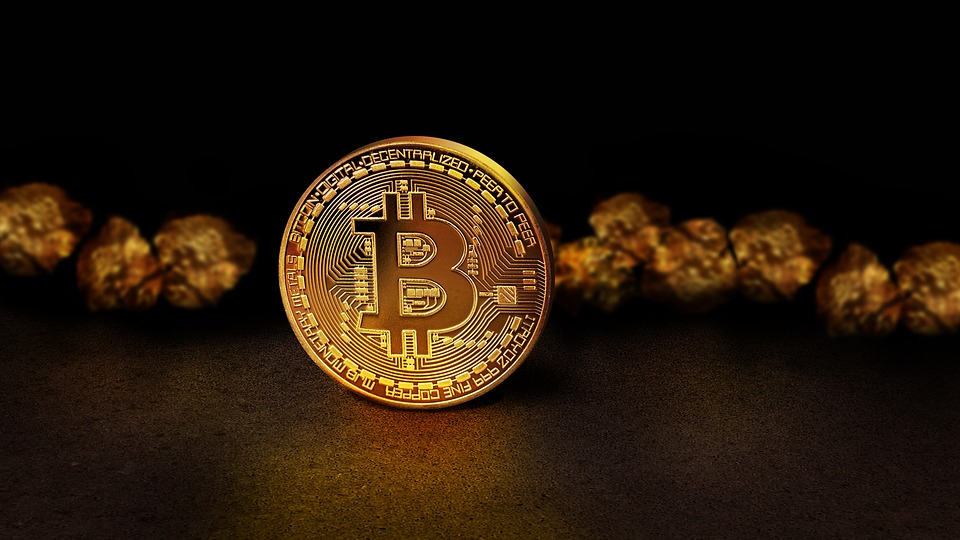
\includegraphics[scale=1]{bitcoin.jpg}\\
\end{frame}

\begin{frame}{Sommaire}
	\tableofcontents
\end{frame}


\section{Presentation du projet}
\begin{frame}{Presentation du projet}
Les technologies liées aux bitcoin et autres cryptomonnaies sont en plein essor, c'est pourquoi il est nécessaire de s'assurer de leur bon fonctionnement. 
\begin{itemize}
    \item Blockchain : technologie de stockage et de transmission d’informations,
    \item Bitcoin : cryptomonnaie, application liée à la blockchain 
    \item Smart Contract : permet de définir et exécuter des contrats de façon automatique sans tierce personne
\end{itemize}
\end{frame}


\section{Objectifs du projet}
\begin{frame}{Objectifs du projet}
\begin{itemize}
    \item Modélisation d'un système de smart contrats
    \item Modélisation d'un contrat sur ce système : Constant-deposit multiparty lotteries on Bitcoin
    \item Définition des propriétés de sécurité
    \item Analyse du système et du protocole pour vérifier les propriétés
\end{itemize}
\end{frame}

\section{Le protocole de lotterie}
\begin{frame}{Le protocole de lotterie} 
\framesubtitle{Arbre de tournoi}
\centering
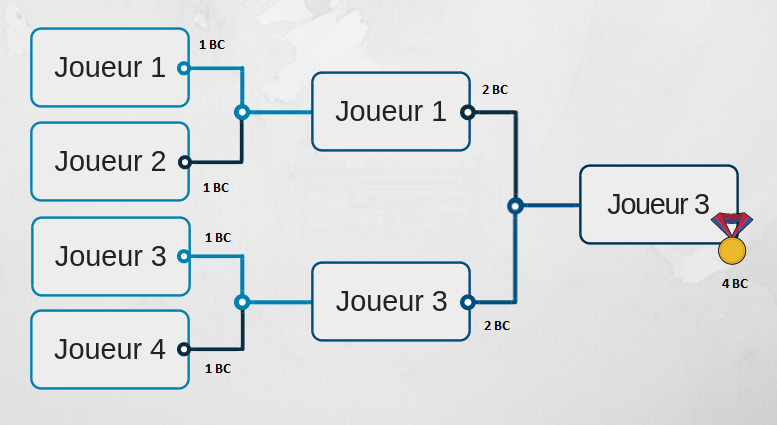
\includegraphics[scale=0.5]{arbre-tournoi.png}\\
\end{frame}

\begin{frame}{Le protocole}

\end{frame}



\section{Tamarin}
\begin{frame}{Tamarin}
\begin{itemize}
    \item Logiciel créé en 2016
    \item Logiciel collaboratif : Analyse symbolique et protocoles de sécurité
    \item 2 grands composant lors de l'écriture d'un protocole :
    \begin{itemize}
        \item Les règles 
        \item Les lemmes
    \end{itemize}
\end{itemize}
\end{frame}


\begin{frame}{Tamarin}
\centering
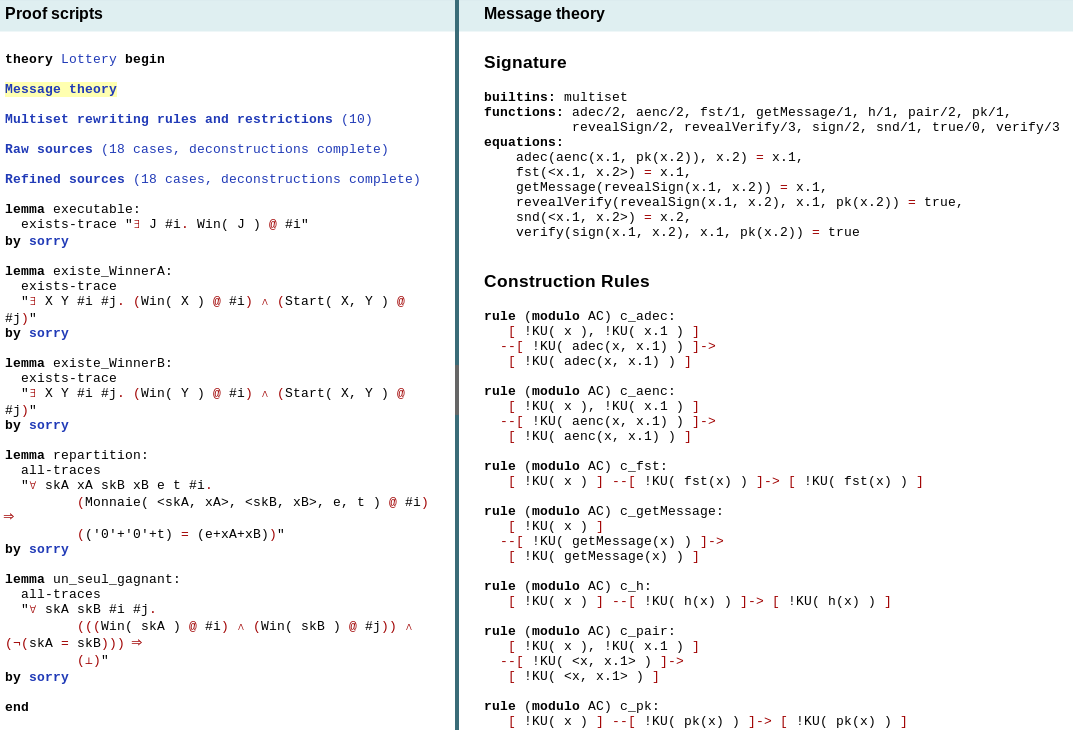
\includegraphics[scale=0.20]{Tamarin1erePage.png}\\
\end{frame}

\begin{frame}{Arbre Tamarin}
\centering
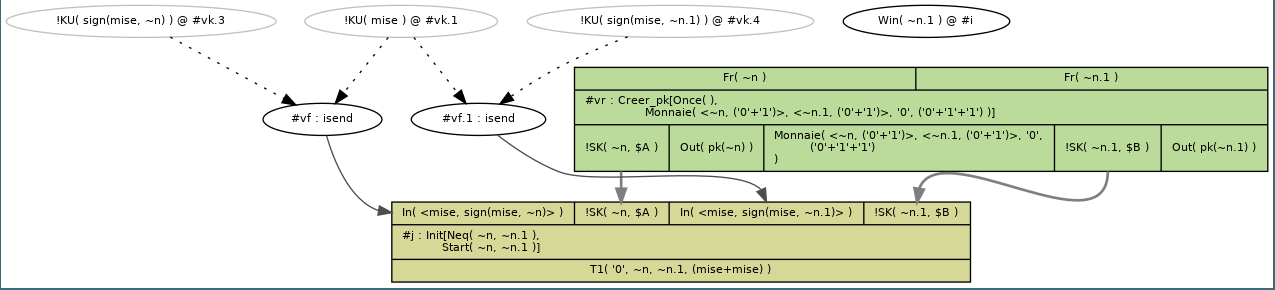
\includegraphics[scale=0.25]{ArbreIntermediaire.png}\\
\end{frame}

\section{Conclusion}
\begin{frame}{Conclusion}
\begin{itemize}
    \item Modélisation d'une exécution du protocole avec des propriétés simples
    \item Modélisation pour 2 joueurs
\end{itemize}
Pour aller plus loin : \\
\begin{itemize}
    \item Garantir qu'aucun joueur ne peut quitter la partie en récupérant son argent
    \item 
\end{itemize}
\end{frame}

\begin{frame}
\Huge Merci de votre attention
\end{frame}

\end{document}